\documentclass[10pt,a4paper]{article}
\usepackage[latin1]{inputenc}
\usepackage[margin=1in]{geometry}
\usepackage{amsmath}
\usepackage{amsfonts}
\usepackage{amssymb}
\usepackage{graphicx}

%\begin{table}[h!]
%		\centering
%		\begin{tabular}{l l l}
%			r1c1 & r1c2 & r1c3 \\
%			r2c1 & r2c2 & r2c3 \\
%		\end{tabular}
%		\caption{Subsystem Specifications}
%		\label{tab:example}
%\end{table}

%\begin{equation}
%	D = \frac{1}{2} \rho V^2 C_D S
%	\label{eq:example}
%\end{equation}

%This is a reference to Table \ref{tab:example}. This is a reference to Figure \ref{fig:example}. This is a reference to Equation \ref{eq:example}. \\ \\ This is a citation \cite{example}. 

%\begin{itemize}
%	\item Overall function of the system
%	\item Constraints from other components of the rocket
%\end{itemize}


\begin{document}
\section{Wireless Ground Communications}
\begin{figure}[h!]
	\centering
	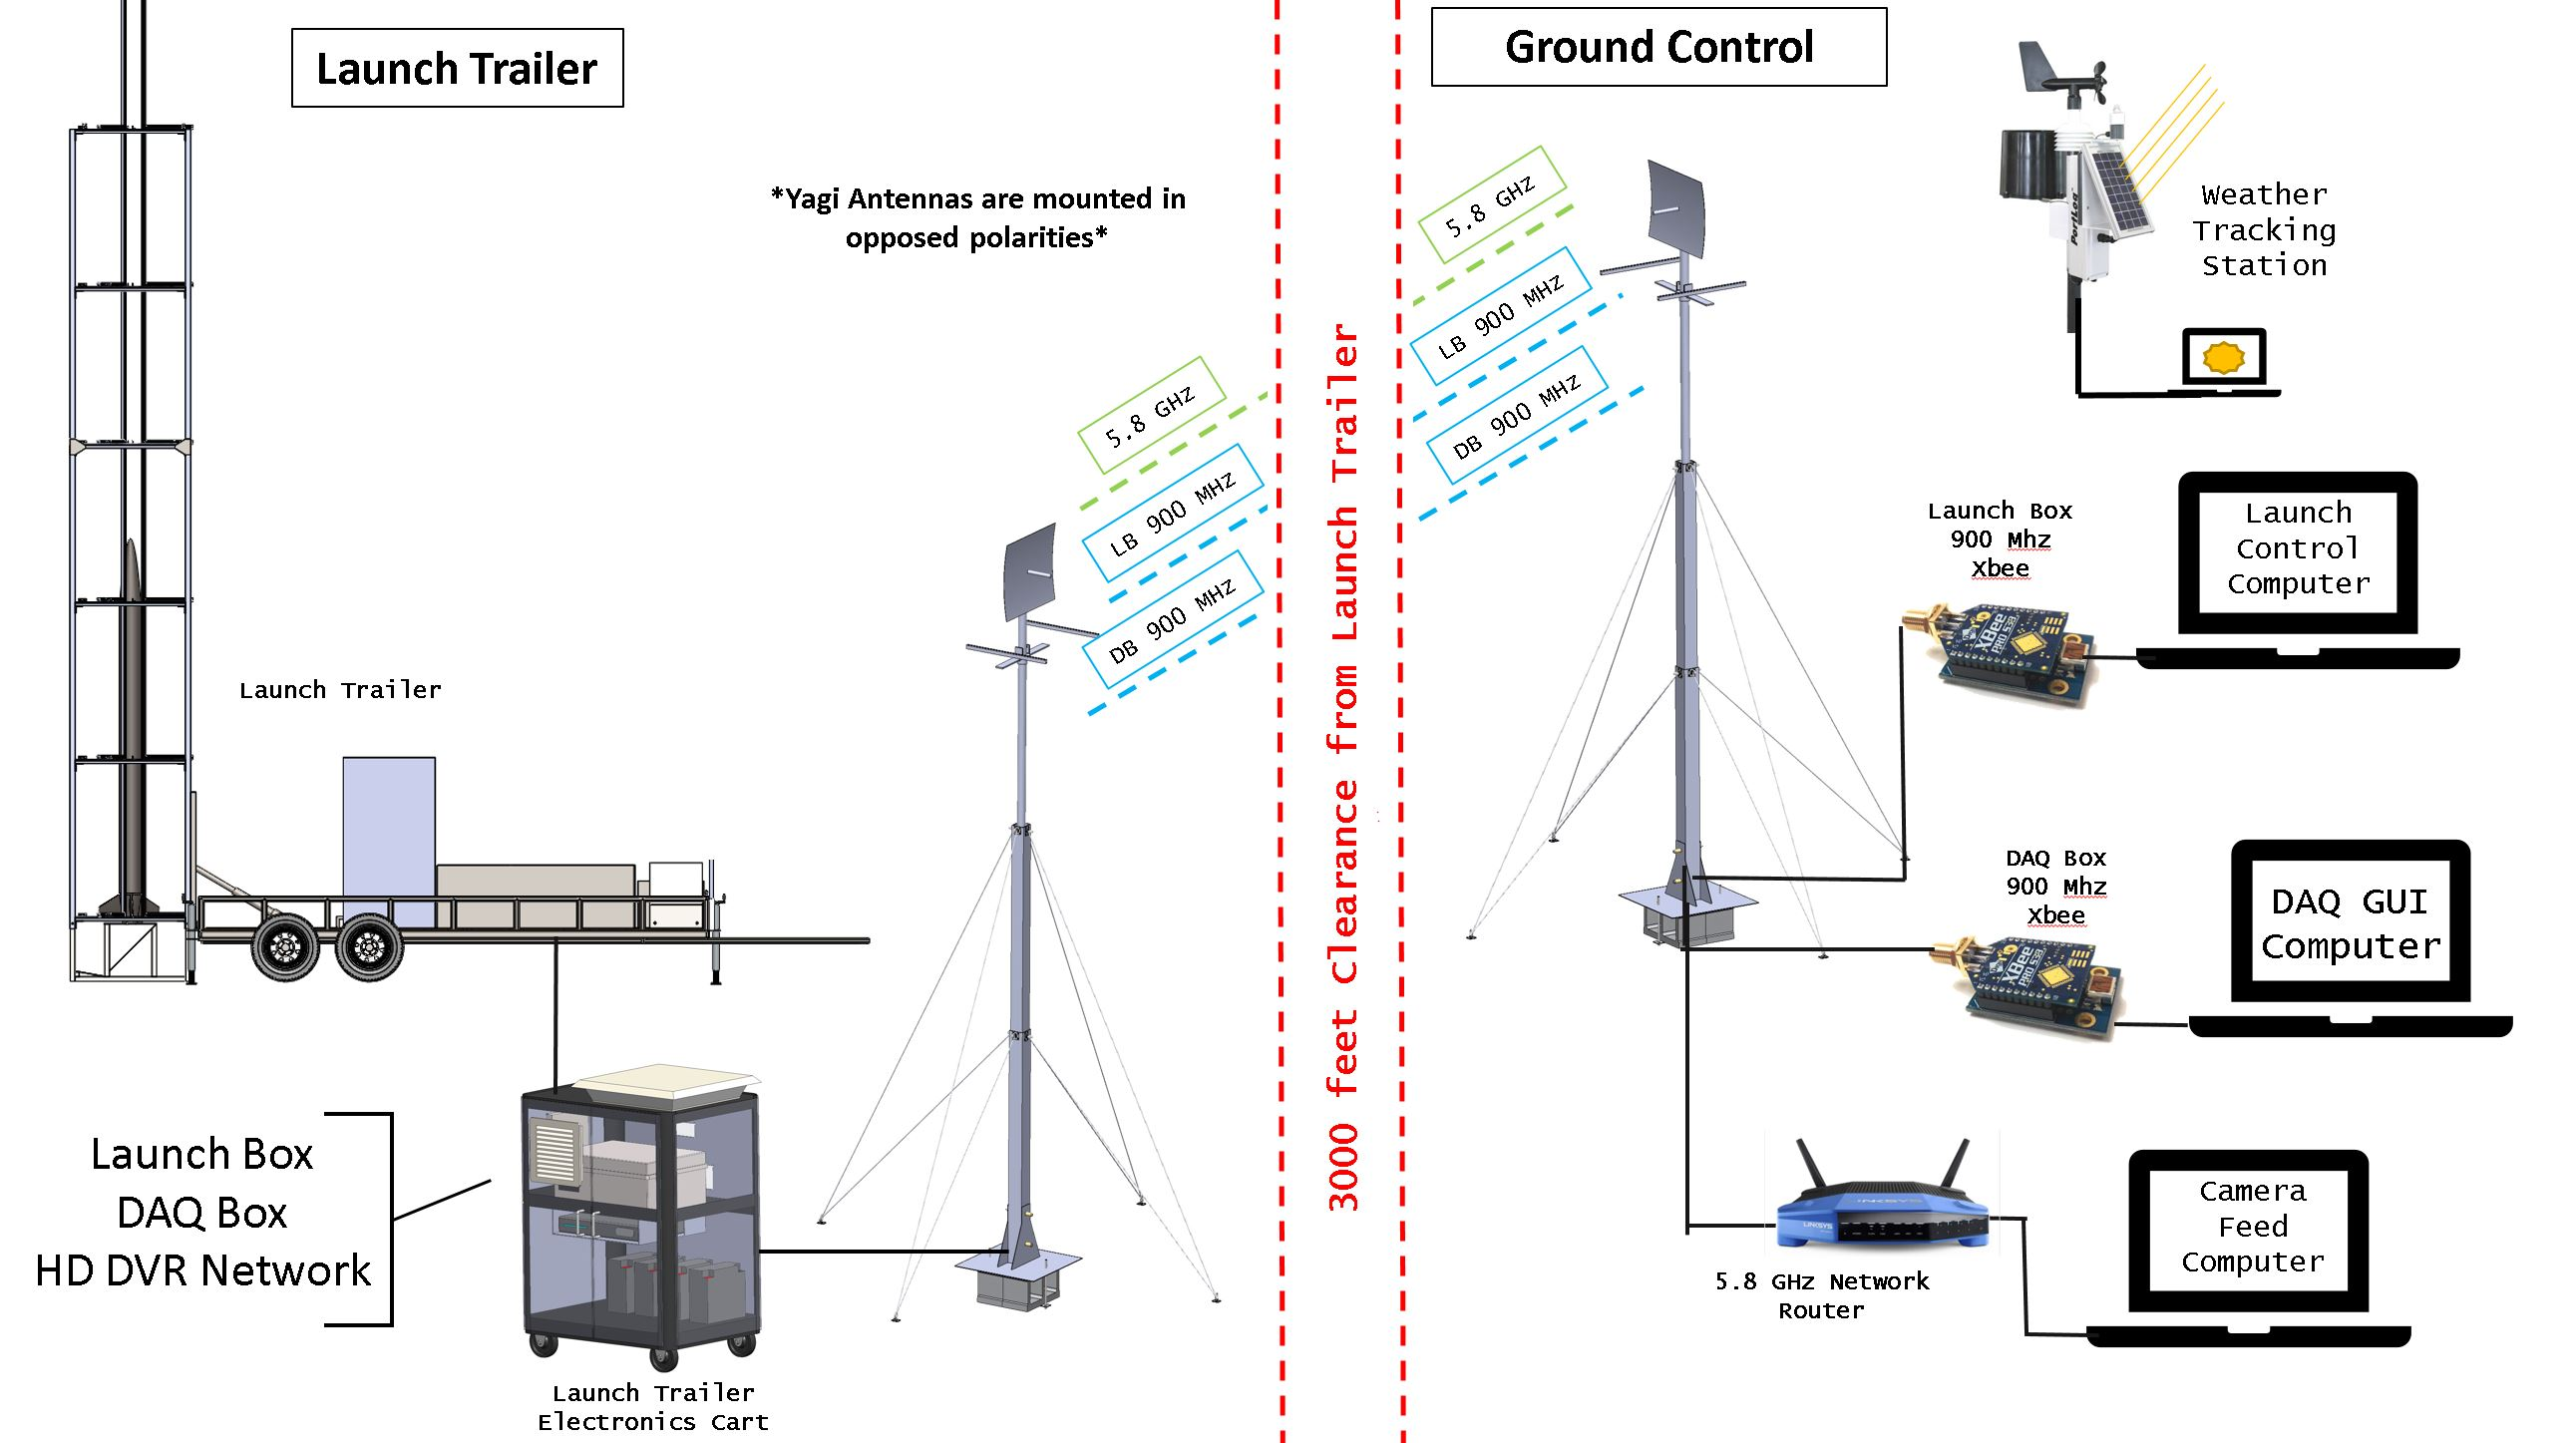
\includegraphics[width=1\textwidth]{./figs/GroundComsOverview.jpg}
	\caption{Wireless Ground Communications Simplified System Overview}
	\label{fig:example}
\end{figure}


\subsection{Overview}
The wireless ground communications system is structured by three Point to Point (PTP) connections in between the launch box, data acquisition box, and Amcrest DVR camera system. The transmissions of the launch and data aquisition box are both sent with Yagi Uda antennas operating at 900 MHz with opposed polarities. The Amcrest DVR camera system operates on a wireless Local Area Network (LAN) with two 5.8 GHz wireless routers at each end transmitting and recieving on high gain parabolic antennas.\\
The purpose for having this communication system is for all the processes required for recording data, filling, and igniting the rocket's hybrid engine along with having a live camera feed of the launch tower and adjacent systems. Considering the importance of the system in launching rockets off the pad, the strongest aspects taken into consideration in the design of ground communications are safety and reliability.

\subsection{Launch Box}
\begin{figure}[h!]
	\centering
	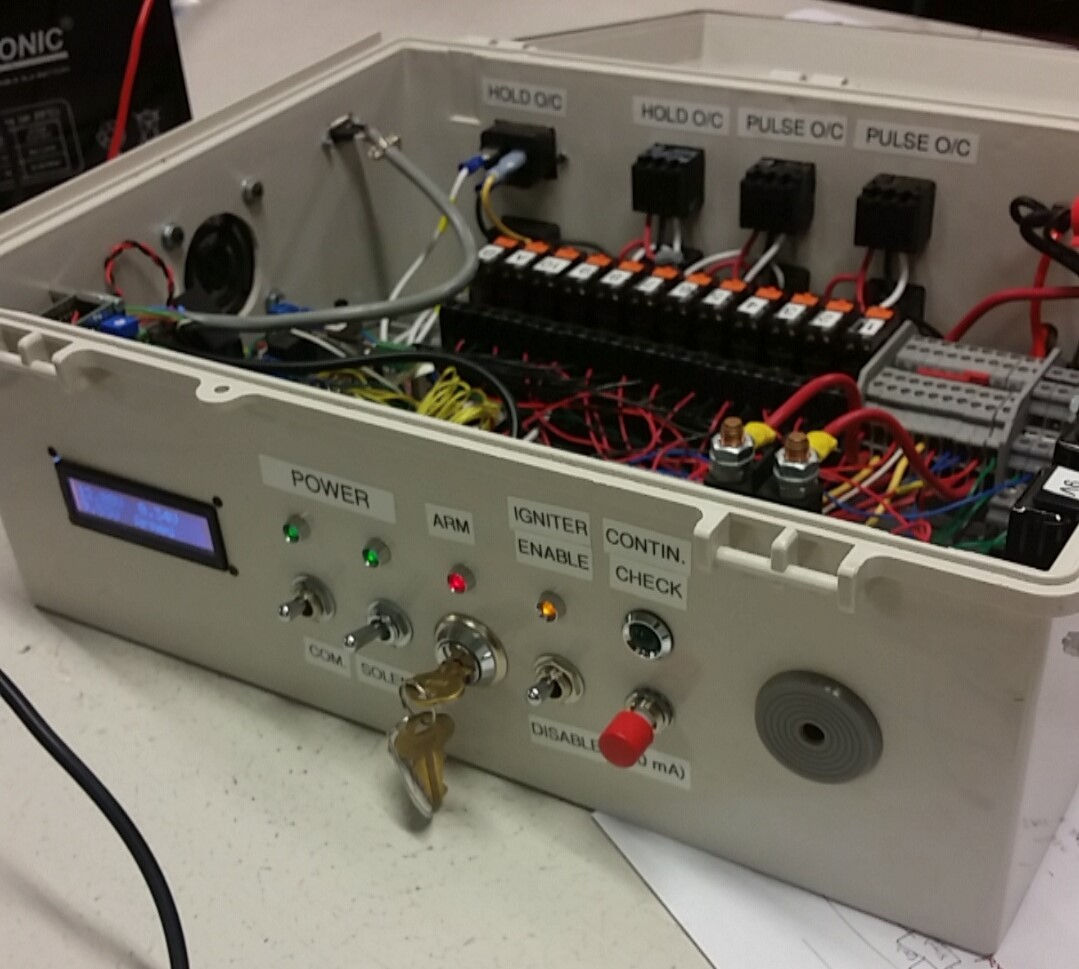
\includegraphics[width=.3\textwidth]{./figs/LaunchBox.jpg}
	\caption{Launch Box Remote Relay System}
	\label{fig:example}
\end{figure}
\subsubsection{Design}
The launch box in essence is a remote relay system for actuatuing solenoids and communicating with the onboard avionics of the rocket. The pseudo-serial connection created by the Digi Xbee-Pro 900 HP is transmitted through a Yagi Uda antenna with horizontal polarization for a PTP connection with another Xbee-Pro 900 HP located at ground control. The ground control computer can then send commands to the launch box for filling and igniting the rocket.\\

Some of the launch box features include:
\begin{itemize}
	\item Continuity test on ignitor, both remotely and on site of launch tower
	\item Remote and on-site arming of igniter and solenoids
	\item 6 Solenoid Channels with 2 Auxillary Relays
	\item Communication with onboard avionics
\end{itemize}
Power for the launch box will be supplied by two sealed lead acid rechargable 12V 18Ah DC batteries, one for system power and one for igniter power, with a conservative expected battery life of around 9 hours.
\subsubsection{User Interface}
The primary interface from ground control to the launch box consists of a graphical user interface (GUI) which rapidly translates data packets being sent through the Xbee serial connection. The launch box GUI can be used to both send commands and display data in real time rolling graphs and gauges. The back up interface utilized to send commands and recieve information from the launch box is through the set up of a serial connection through PuTTy at 9600 bits per second which utilizes a considerably slower data rate but with the added reliability of direct commands through serial port connection to the Arduino Mega in the launch box.\\
\subsubsection{Wireless Interference Considerations} \label{PolarizationMismatch}
 Considering that the launch box is transmitting at a close frequency with the data acquisition box from the launch trailer, one of the methods used to limit cross-interference across either Yagi antenna is through the use of opposed antenna polarization.
\begin{figure}[h!]
	\centering
	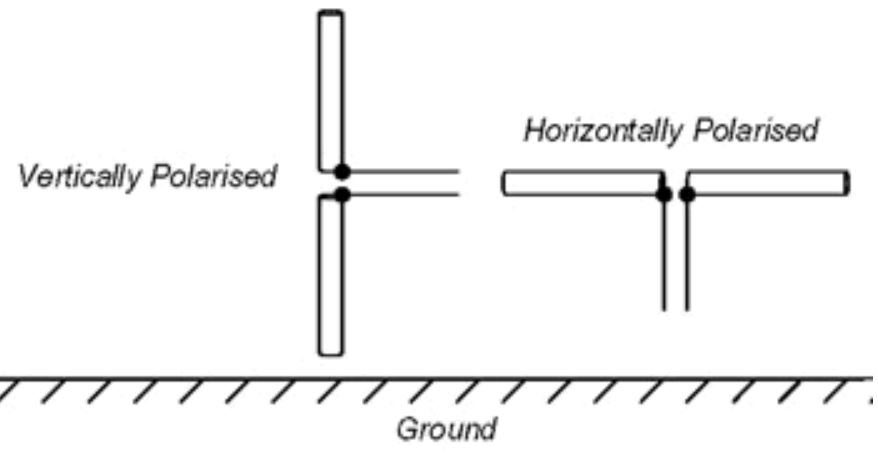
\includegraphics[width=.35\textwidth]{./figs/AntennaPolarization.jpg}
	\caption{Horizontal and Vertical Dipole Polarization}
	\label{fig:polarization}
\end{figure}
With the act of mounting the launch box Yagi antenna in a vertically polarized orientation and the DAQ box Yagi antenna in a horizontally polarized orientation will create a maximum theoretical mismatch of 30 dBi (Figure: \ref{fig:Mismatch}). Of course in our antenna tower the pair of Yagi antennas are mounted around 6.06 quarter-wavelengths apart (quarter-wavelength calculation \ref{eq:QuarterWave} [in]), so some cross-interference might still be possible but will also be curtailed by software multiplexing native to the Xbee 900 HP modules used by both antennas.
\begin{figure}[h!]
	\centering
	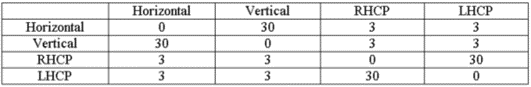
\includegraphics[width=.6\textwidth]{./figs/PolarizationTable.png}
	\caption{Theoretical Polarization Mismatch of Different Types}
	\label{fig:Mismatch}
\end{figure}
Changes were made HERE
\begin{equation}
	\frac{\lambda}{4}= \frac{c}{f}*\frac{1}{4}
	\label{eq:QuarterWave}
\end{equation}


\subsection{Data Acquisition Box}
\subsubsection{Design}
The data acquisition box is a in essence an Arduino Mega microcontroller that takes in a variety of analog and digital signals which are then transmitted to ground control in order to provide a live data feed of various systems on the launch trailer. The purpose for implementing this new data acquisition box for the SRT-5 year is to prevent a bottle-neck of data, which would happen if all data were to be sent through the launch box alone. Some of the signals that the data acquisition box will recieve from the launch trailer system includes:
\begin{itemize}
	\item Fill Tank Pressure Transducer (Absolute)
	\item Fill Tank Thermocouple and Ambient Thermocouple
	\item Fill Tank Load Cell and Rocket Pad Load Cell
	\item Wind Speed Anemometer and Weathervane
\end{itemize}
Power for the data acquisition box will be supplied by a sealed lead acid rechargable 12V 18Ah DC battery with a conservative expected battery life of around 19 Hours. 
\subsubsection{User Interface}
The Xbee module within the data acquisition box will complete a PTP pseudo-serial connection to the DAQ computer located at ground control which will funnel data into the launch trailer GUI. Furthermore, switches located at the data acquisition box will enable operators to power the system on-or-off.
\subsubsection{Wireless Interference Considerations}
The wireless transmission of the data acquisition box will be using the same system as the previously mentioned launch box with a Xbee 900 HP module and Yagi directional antenna, however, the Yagi antenna will be mounted in a horizontally polarized orientation in order to maintain an opposed polarization with the launch box antenna as previously explained with the concept of polarization mismatch in section \ref{PolarizationMismatch}.




\subsection{Camera System}
\subsubsection{Design}
The HD DVR System by Amcrest is a standard 4-channel security camera system that is being used for multiple live feed camera angles of the launch trailer. The Amcrest system has multiple networking capabilities including live feed monitoring over PTP network LAN connection, which is the capability our team will be utilizing for wireless camera feed. The Amcrest DVR will utilize two 5.8 GHz wireless network routers with high gain commercial parabolic antennas to complete a PTP connection spanning an average of 3000 feet.\\
\begin{figure}[h!]
	\centering
	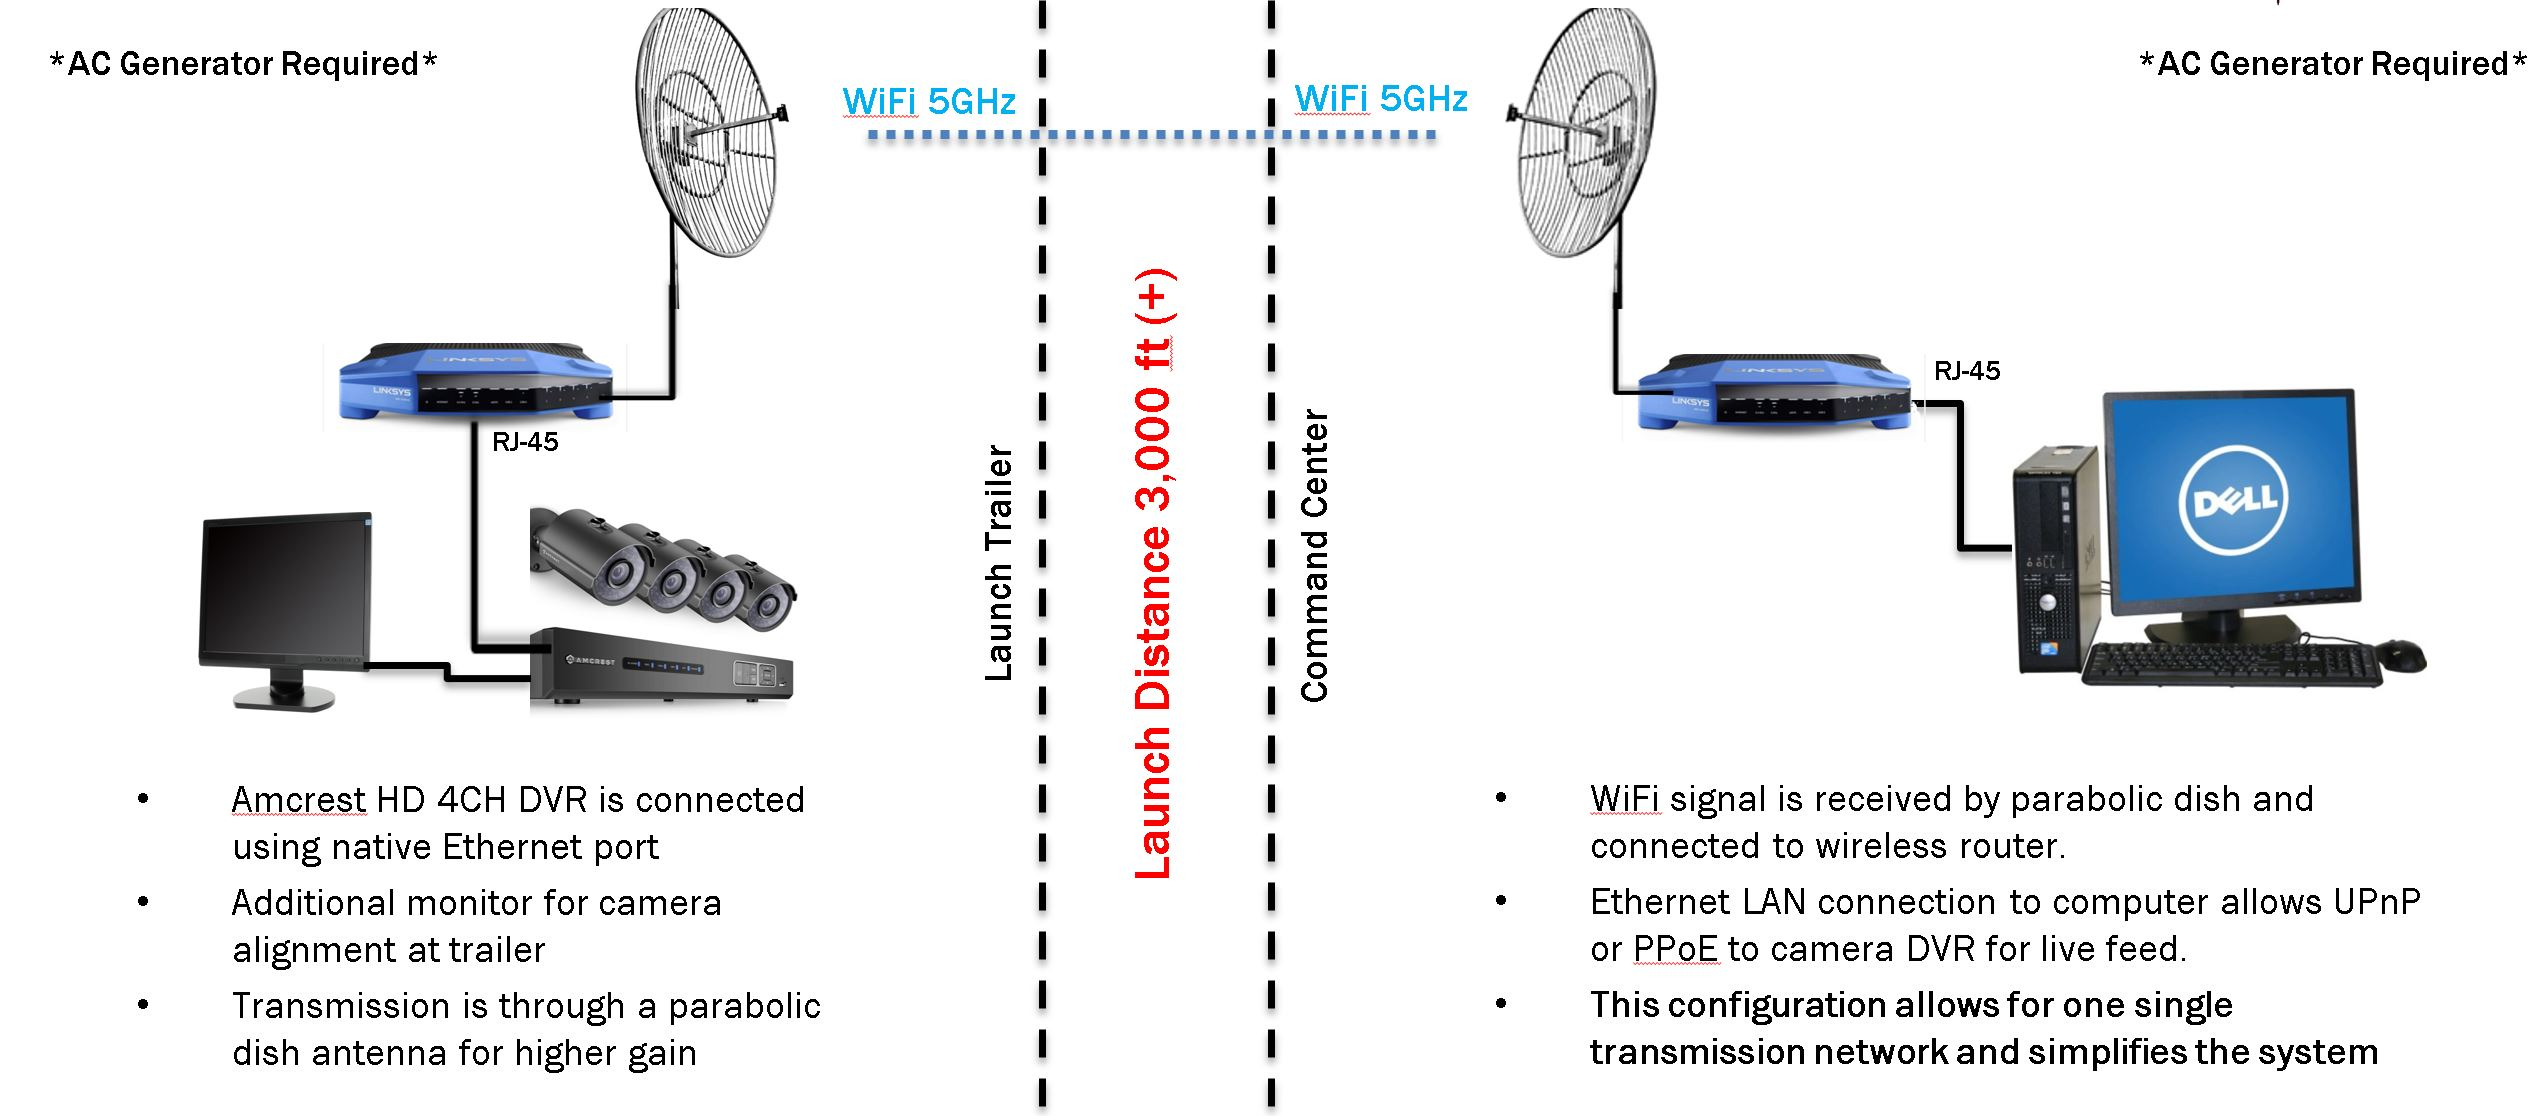
\includegraphics[width=1\textwidth]{./figs/CameraSystemSetup.jpg}
	\caption{Simplified Camera System Diagram}
	\label{fig:example}
\end{figure}
Previous attempts for implementing a live camera feed of the launch trailer have included a system of separate transmitters and antennas for each individual camera that was found to produce interference between channels when tested. The advantage to using the Amcrest DVR network capabilities as opposed to individual transmitters is the fact that it simplifies the overall transmission pattern down to one signal on a parabolic dish while also cutting down on the overall cost of purchasing individual transmitters.
\subsection{User Interface}
Due to the use of the network capabilities of the Amcrest HD DVR system the option to utilise Point-to-Point Protocol Over Ethernet (PPPoE) or Universal Plug-n-Play (UPnP) is availaible through a wireless LAN network. Regardless of the communication protocol the operator at ground control will utilize a computer connected to the PTP wireless router for access to the Amcrest HD DVR through a LAN browser for live camera feed.
\begin{figure}[h!]
	\centering
	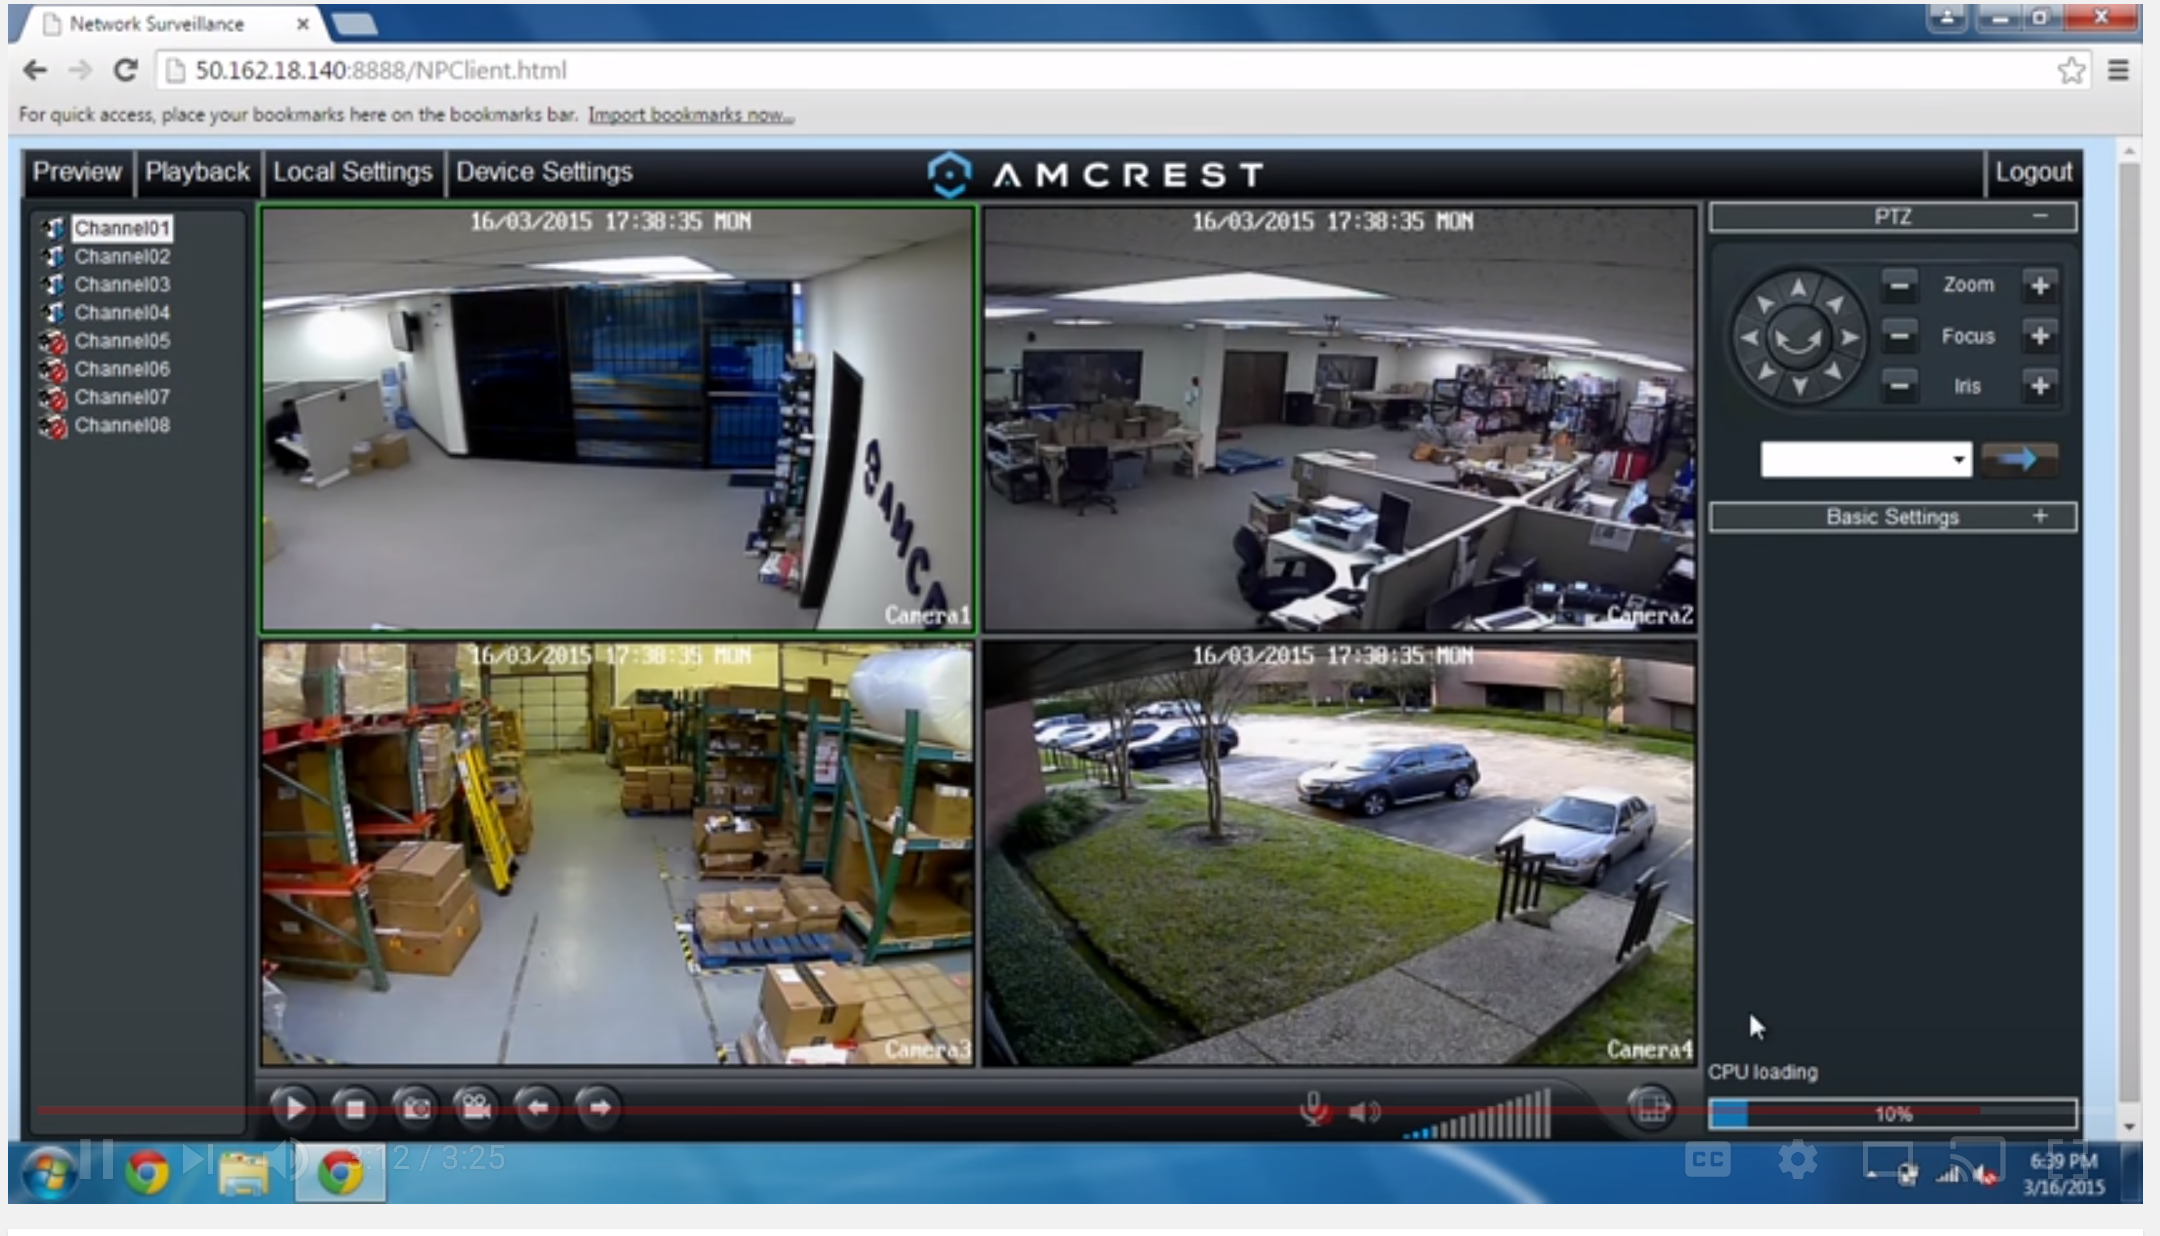
\includegraphics[width=.9\textwidth]{./figs/AmcrestBrowser.png}
	\caption{Example of LAN Browser Live Feed}
	\label{fig:example}
\end{figure}
\subsubsection{Wireless Interference Considerations}
The parabolic antennas that will be implemented with the 5.8 GHz wireless routers are commercial parabolic antennas advertised at 27 dBi gain for point-to-point applications. Normally these parabolic antennas in ideal conditions can have a range of around 3 Miles (15,840 ft) with the operating 5.8 GHz frequency which is more than enough gain for a transmission range of 3,000 ft with expected line of sight over any obstructions. Due to the fact the transmission range at competition is so short compared with the ideal transmission range, our line-of-sight PTP application is expected to suffer little to no signal loss or fade during use.\\
Another possible venue of interference also considered, is that of other 5.8 GHz networks around ground control or in between the transmission range. The mitigation of such interference however, can be taken care of by analzying nearby frequencies with a Wi-Fi spectrum analyzer application and shifting both wireless routers to less occupied bands. Furthermore, the wireless routers internal WiFi Protected Access Pre-Shared Key (WPA-PSK) will also prevent any unregistered users from accessing the wireless PTP local area network (LAN).



\subsection{Antenna Towers}
\begin{figure}[h!]
	\centering
	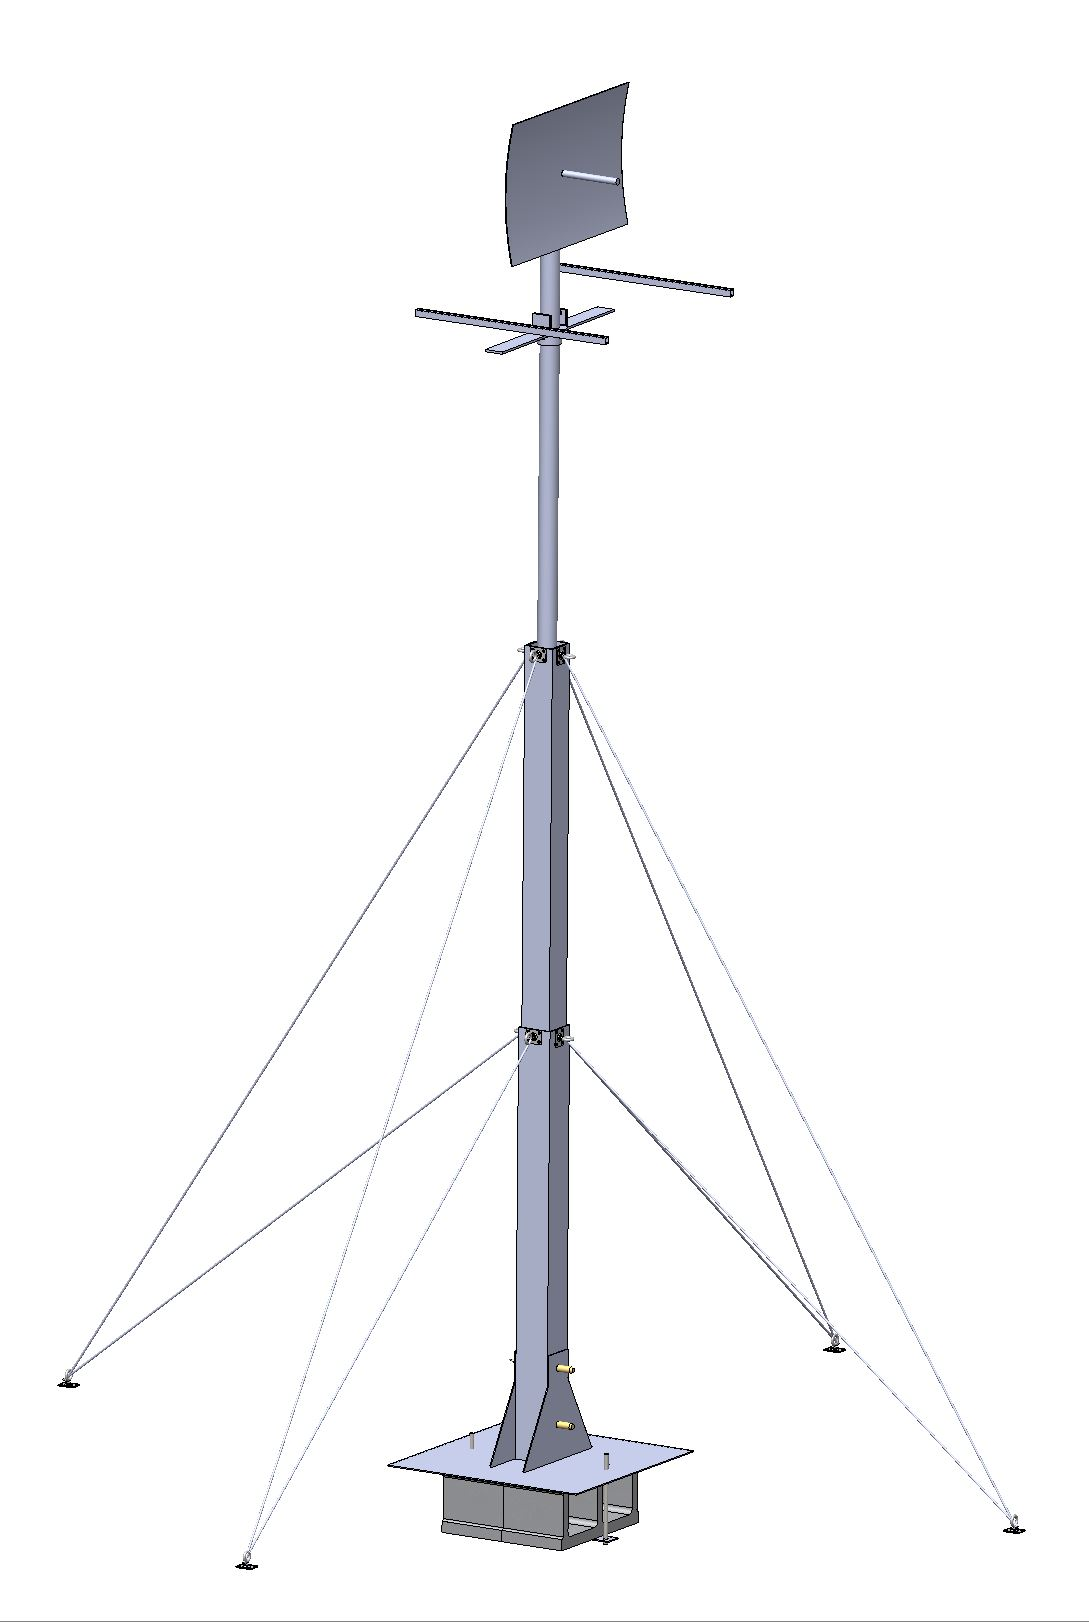
\includegraphics[width=.5\textwidth]{./figs/AntennaMast.jpg}
	\caption{Antenna Tower CAD Model}
	\label{fig:example}
\end{figure}
\subsubsection{Design}
The design for the antenna towers utilized for wireless ground communications will fulfill two important requirements needed for ideal antenna placement and transmission. 
\begin{itemize}
	\item 1. Steady antenna Line-of-Sight for Point-to-Point transmission
	\item 2. Increase in Radio Horizon above obstructions located near launch trailer and ground control
\end{itemize}
The height of the antenna towers need to be a minimum of 12 feet in order to account for the height of desert foliage along with the potential elevation differences in between the launch trailer antenna tower and ground control antenna tower. This height was calculated by a measurement of foliage during IREC 2017 in Space Port, New Mexico along with the a conservative estimate for terrain height difference.
\subsubsection{Alignment}
Considering the distance of transmission in between both antenna towers (3,000 ft), alignment for the parabolic antenna and two yagi antennas will be done with compass measurements of both antenna tower locations along with angle measurements of antenna vertical direction. Final alignment adjustments will be also be performed with an active transmission in order to ensure proper signal calrity.
\subsubsection{Manufacturing}
The manufacturing of the antenna towers will require stock 6061-T6 aluminum alloy sections along with steel guy-wire and fasteners for the vertical stability of the antenna towers. The assembly procedure of the antenna towers will simply require raising telescoping sections of the tower and pinning them in place with trailer hitch pins at set distances along with driving stakes at set distances of the antenna tower base for guy-wire placement.



\subsection{Yagi Antennas}
The Yagi antennas utilized consist of aluminum booms with fully insulated antenna elements and fully insulated folded dipole radiators. Both Yagi antennas will operate on the 900 MHz band with eight parasitic elements and one reflector with the pair of antennas mounted in opposing polarizations. The concept of opposing polarization mounts and its benefits are discussed in section \ref{PolarizationMismatch}.



\subsection{Parabolic Antennas}
The antennas which we will be using for the 5.8 GHz band of the wireless routers in our PTP transmissions will be the L-COM HG5827EG commerical parabolic antennas sold by ISP Supplies. While manufacturing our own parabolic antennas was in consideration in order to cut-down on costs, the conclusion we arrived to after a feasibility investigation were that the material costs for a do-it-yourself (DIY) parabolic antenna would closely match the price of a commercial parabolic antenna and the DIY antennas would certainly be less efficient than a commerical grade antenna due to manufacturing error.
\begin{figure}[h!]
	\centering
	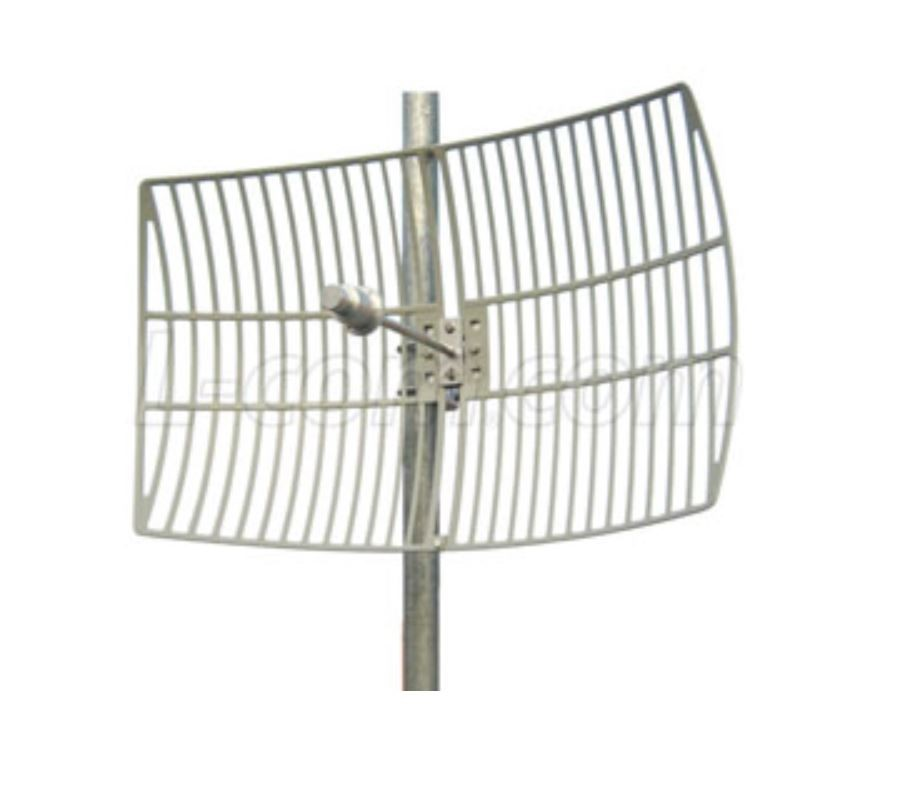
\includegraphics[width=.75\textwidth]{./figs/ParabolicAntenna.jpg}
	\caption{L-COM HG5827EG}
	\label{fig:example}
\end{figure}



\subsection{Testing}
Taking into consideration the nature of wireless transmissions, many of the testing procedures for all systems involved in wireles ground communication involve repeated and varied tests of the system in different conditions in order to verify design expectations. One aspect of testing and review which is new to SRT-5, is the inclusion of testing antennas with lab equipement in conjunction with Texas A\&M University Faculty. Lab testing all manufactued antennas including the comercially pruchased antennas will allow a deeper insight into the true performance capabilities of the ground communications system and where possible interferences can be expected.



\begin{thebibliography}{10}
	\bibitem{example}
	Joseph J. Carr, George W. Hippisley,
	"Practical Antenna Handbook", McGraw Hill 5th Edition,
	United States, 2012

	\bibitem{example}
	Air-Stream.org
	"Antenna Polarization" [Figure \ref{fig:polarization}]
	United States, 2017
	
\end{thebibliography}

\end{document}